\documentclass[letterpaper]{article}
\usepackage{natbib,alifexi}
\usepackage{float}
\usepackage{amsmath}
\usepackage{array}

\title{A Shortest Path Algorithm Used to Solve Optimal Bids in an Electricity Spot Market}
\author{G\'erard Tio Nogueras \\
\mbox{}\\
Universit\'e Libre de Bruxelles, Bruxelles, Belgique\\
gtionogu@ulb.ac.be}


\begin{document}
\maketitle

\begin{abstract}
A good descriptive abstract functions to describe as accurately as possible the content and purpose 
of a research report. It doesn’t  provide results or conclusions of the research. It does incorporate 
key words found in the text and may include the purpose, methods, and scope of the research. Some
people consider it an outline of the work, rather than a summary. Descriptive abstracts are usually 
very short—100 words or less.
\end{abstract}

\section{Introduction}

A wholesale energy market is a market for electric power transactions. All the energy producers bid energy units depending on their production capacity. Then the system operator distributes hour shifts to some chosen generators(owned by the energy producers)by increasing value of their price until the demand is met. The really important point is that all generators unit price is that of the most expensive loaded generator. We will call this price, the spot price. Therefore as long as you are cheaper or equal to the final spot price you will be chosen by the operator. Companies try to predict the spot price to sell a maximum quantity of energy at the highest price lower than the future spot price so that they will be chosen over others.
This is the result of the system operator that tries to minimise his expenses.\\ \\
The problem is studied, among others, by Fampa et al.[Bilevel optimization applied to strategic pricing in competitive electricity markets] which presents two different approaches to solve the problem: The first one is a heuristic technique considering a generous dispatching.
The second one is a mixed integer reformulation of the problem used to find the optimal solution and allows the validation of the heuristic approach.\\ \\
The goal of this report is to find faster ways to solve it. By simplifying some of the constraints and changing the dispatching resolution a little bit, we can reduce the problem to a shortest path problem and apply faster algorithms.
\section{The Optimal Bid/Bidding Problem}
The problem studied is the following, we are a company that we will call the leader or L that wants to maximize its profit in a specific environment, a wholesale electric market like described in the introduction, where the leader competes against other companies. The main goal is to find what quantity bids the leader should make and at what prices to maximize its profit.
\subsection{Mathematical presentation of the problem}
Here is the data provided with the problem: \\ \\ 
\begin{tabular}{ll}
$d$ & The total load needed \\
$g_j$ & The energy production of generator j \\ 
$J$ & Group of all generators \\
$c_j$ & The operating cost of generator j \\ 
\end{tabular}\\ \\
The variables used to model the problem are the following: \\ \\
\begin{tabular}{ll}
$\lambda_j$ & The price bid of a generator j \\ 
$\overline{g}_j$ & The generation capacity bid of generator j \\ 
$\pi_d$ & The spot price \\ 
$R_j$ & The profit of generator j \\ 
$R$ & The net profit of a company E, group of generators $j \in E$ \\
\end{tabular}\\ \\
Companies related variables: \\ \\
\begin{tabular}{ll}
$\lambda_E$ & set of price bids \\
$\overline{g}_E$ & quantity bids \\ 
\end{tabular}\\ \\
The problem of the system operator can be formulated as the following linear program:\\ \\
\begin{equation}
min_{g_j} \ \sum_{j \in J} \lambda_j g_j
\end{equation}\\
this is the total cost for the quantity bids chosen by the system operator.\\ \\
s.t.
\begin{equation}
\sum_{j \in J} g_j = d  \label{eqn:load}
\end{equation}\\
The sum of all the quantity bids must fulfil the demand.\\
\begin{equation}
g_j \leq \overline{g}_j, j \in J \label{eqn:g_j}
\end{equation}
A quantity bid for a generator cannot exceed the generator's capacity.\\ 
\begin{equation}
g_j \geq 0, j\in J
\end{equation}
The quantity bid for the generator j must be positive.\\ \\
Let $\pi_d$ denote the dual variable of constraint (\ref{eqn:load}) and $\pi_{g_j}$ that of constraint (\ref{eqn:g_j}).\\
This model shows how the system operator wants to minimize his expenses.
We can add another interesting value useful for future purposes, the profit for each generator j :\\ \\
$R_j = (\pi_d - c_j)g_j, j \in J$ \\ \\
The profit for each generator is the amount of energy sold times the difference of the price it sold and its cost of production. \\ 
Then comes the objective function that the leader(L) wants to maximize and which represents its profit. First we have to introduce more variables to model the simultaneous competition between all the companies, the company L, uses a set of scenarios where competitors actions are represented. New variables are introduced for the bidding under uncertainty: \\ \\
\begin{tabular}{ll}
$p_s$ & The probability of a scenario $s \in [1,...,S]$\\
$S$ & Set of scenarios \\
$ER(\lambda_E,\overline{g}_E)$ & The expected profit\\
$g^*_j$ & The maximum capacity of \\
 & production of generator j \\
$\pi^s_d(\lambda_E,\overline{g}_E)$ & Spot price for a specific scenario\\ 
$g^s_j(\lambda_E,\overline{g}_E)$ & energy production of a generator j \\
& for a specific scenario \\
\end{tabular}\\ \\
With the new variables the objective function for the generators becomes:\\ \\
\(\displaystyle max_{\lambda_E , \overline{g}_E}$ $ER(\lambda_E,\overline{g}_E)\) = \(\displaystyle \sum_{s \in S} p_s R^s (\lambda_E , \overline{g}_E)\)\\ \\
where\\ \\
\(\displaystyle R^s (\lambda_E , \overline{g}_E) = \sum_{j \in E}(\pi_d^s(\lambda_E , \overline{g}_E) - c_j)g_j^s(\lambda_E , \overline{g}_E)\)\\
is the profit of company E in scenario s and $g^*_j$ is the maximum capacity of production of generator j.\\\\
s.t.\\ \\
$\overline{g}_j \leq g^*_j, j \in E$ \\ \\
Fampa et al.[\c{Fampa M.,2007}] go on formulating the global problem  with the objective function of the company L we represent and the system operator function. Afterwards they introduce two models based respectively on fixed prices and fixed quantities.
Finally they present their different solutions to solve these models.

\section{Presentation of the new formulation}
\begin{tabular}{ll}
$s \in S$ & the set of all scenarios, \\
$j \in J$ & the set of all generators we control, \\
$j \in J^c$ & the set of all generators of the competitors, \\
$i \in I$ & the set of all possible bid prices.
\end{tabular}\\ \\
The model parameters:\\ \\
\begin{tabular}{ll}
$p_s$ & the probability that the scenario $s$ will be realised, \\
$d_s$ & the total demand in the scenario $s$, \\
$\lambda^c_{s,j}$ & the price bid by the competitors \\
 & in the scenario $s$ for their generator $j$, \\
$\bar{g}^c_{s,j}$ & the quantity bid by the competitors \\
& in the scenario $s$ for the generator $j$, \\
$g^{c*}_j$ & the maximum quantity which can be produced \\
& by the competitors generator $j$, \\
$g^*_j$ & the maximum quantity which can be produced \\
 & by our generator $j$, \\
$c_j$ & the operating cost to produce one unit of energy \\
 & by our generator $j$.
\end{tabular}\\ \\

The model variables:

\begin{tabular}{ll}
$R_s$ & our profit during scenario $s$, \\
$R$ & our average profit for all scenarios, \\
$\pi_s$ & the spot price during scenario $s$, \\
$\lambda_{j}$ & the price bid by us for our generator $j$, \\
$\bar{g}_{j}$ & the quantity bid by us for our generator $j$, \\
$g^c_{s,j}$ & the actual quantity produced \\
  & by the competitors generator $j$ during scenario $s$, \\
$g_{s,j}$ & the actual quantity produced by \\
 & our generator $j$ during scenario $s$.
\end{tabular} \\ \\
The formulation is as follows:
\begin{equation}
\max R, \\
\end{equation}
s.t. \\ \\
\begin{equation}
R = \sum_{s \in S} p_s R_s
\end{equation}
The total profit is equal to the sum of the scenario's profit associated with the probability.\\
\begin{equation}
R_s = \sum_{j \in J} \left(\pi_s - c_j\right) g_{s,j} \ \ \forall s \in S
\end{equation}
The profit associated with a specific scenario is equal to the sum of our quantity bids sold for this scenario times the difference of the spot price for this scenario and the cost of production for the generator j.\\
\begin{equation}
\sum_{j \in J} g_{s,j} + \sum_{j \in J^C} g^c_{s,j} = d_s \ \ \forall s \in S
\end{equation}
The sum of the quantity bids for our generators and those of our competitors must be equal to the demand.\\
\begin{equation}
g^c_{s,j} \ge 0 \ \  \forall s \in S, j \in J^c
\end{equation}
\begin{equation}
g^c_{s,j} \le \bar{g}^{c}_j \ \  \forall s \in S, j \in J^c
\end{equation}
\begin{equation}
\bar{g}_{s,j} \ge 0 \  \ \forall s \in S, j \in J
\end{equation}
\begin{equation}
\bar{g}_{s,j} \le g^*_j \ \  \forall s \in S, j \in J
\end{equation}
\begin{equation}
g_{s,j} \ge 0 \ \  \forall s \in S, j \in J
\end{equation}
\begin{equation}
g_{s,j} \le \bar{g}_j \ \   \forall s \in S, j \in J
\end{equation}
The quantity bids must be positive and inferior or equal to the capacity of their associated generator j.\\
\begin{equation}
\lambda^c_{s,j} < \pi_s \rightarrow g^c_{s,j} = \bar{g}^{c}_j \ \ \  \forall s \in S, j \in J^c
\end{equation}
\begin{equation}
\lambda^c_{s,j} > \pi_s \rightarrow g^c_{s,j} = 0 \ \ \  \forall s \in S, j \in J^c
\end{equation}
\begin{equation}
 \lambda_{j} < \pi_s \rightarrow g_{s,j} = \bar{g}_j \ \ \  \forall s \in S, j \in J
\end{equation}
\begin{equation}
\lambda_{j} > \pi_s \rightarrow g_{s,j} = 0 \ \ \  \forall s \in S, j \in J
\end{equation}
If a competitor's bid price is inferior to the spot price, then the actual quantity sold is the quantity bid made by the competitor for this generator. If the bid price is higher then the spot price, then no quantity is sold. Same applies for our bids.\\
\begin{equation}
\pi_s \in \left\{ \lambda^c_{s,j} \forall j \in J^c \right\} \cup \left\{ \lambda_j, \forall j \in J \right\} \ \ \  \forall s \in S
\end{equation}\\ \\
The spot price for a specific scenario must be at one of the bid prices given by one of the companies for this scenario.\\ \\
Before discussing the algorithm used to solve this problem, let us introduce two propositions to support the solution.\\ 
The first proposition tries to give more sight to where the optimal bid stands.
\subsection{Proposition 1 - optimal bid price}
The optimal value for each bid price $\lambda_j$ is always equal to one of the possible competitors bid prices $\lambda_{s,j}^c$, assuming that ties are resolved in our advantage.\footnote{Mixed-Integer Programming Formulation, E. Marcott}
There exists an optimal bid price $\lambda_j \in \{\lambda^c_{s,j}: s \in S, j \in J^c \}$
\subsection{Proof}
First we consider that our bids are strictly between two other bids, there are no other bids in between:\\ \\
$\exists s \in S:\lambda_{s,j1}^c < \lambda_j < \lambda_{s,j2}^c$ \\ \\
It is important to note that bid prices are in ascending order:\\
$ \{ \lambda_{s_1}, ..., \lambda^c_{s,j_1}, \lambda_j, \lambda^c_{s,j_2}, ...,\lambda_{s_n} \}$
where $\lambda_{s_1}$ is the lowest bid price for a specific scenario s and $\lambda_{s_n}$ is the highest bid price for the same scenario.
Now lets prove that by increasing $\lambda_j$ to $\lambda_{s,j2}^c$ the profit $R$ would either increase or remain constant. We will prove this by analysing the three different possible cases. The reason there are only 3 cases which are  $\lambda_{s,j2}^c \leq \pi_s$, $\lambda_{s,j1}^c \geq \pi_s$ and $\lambda_j = \pi_s$, is because the profit is mainly influenced by the spot price and for a given bid price the spot price can either be lower, higher or equal to the bid price.
\begin{itemize}
\item Case 1: $\lambda_{s,j2}^c \leq \pi_s$ \\

\begin{figure}[H]
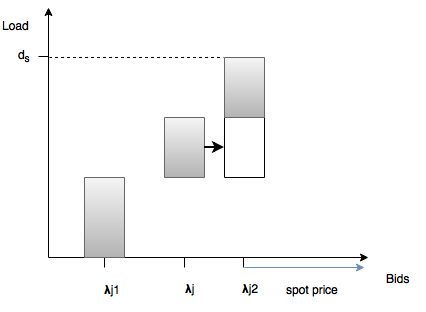
\includegraphics[scale=0.5]{../documentation/p1_c1.png}
\caption{Spot price higher then $\lambda_{s,j2}^c$ bid. If$\lambda_j$ becomes $\lambda^c_{s,j_2}$ since the spot price is higher then the price offered by $\lambda_{s,j2}$, changing to $\lambda_{s,j2}$ will not change the profit $R_s$.}
\end{figure}
\item Case 2: $\lambda_{s,j1}^c \geq \pi_s$ \\

\begin{figure}[H]
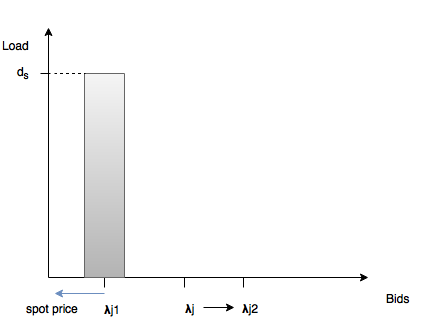
\includegraphics[scale=0.5]{../documentation/p1_c2.png}
\caption{Spot price lower then $\lambda_{s,j1}^c$ bid. Since the spot price is lower than $\lambda_{s,j1}$ that means that the total load is achieved for the values under $\lambda_{s,j1}$, so changing $\lambda_{s,j1}$ to $\lambda_{s,j2}$ will have no effect on $R_s$. }
\end{figure}
\item Case 3: $\lambda_j = \pi_s$ \\

\begin{figure}[H]
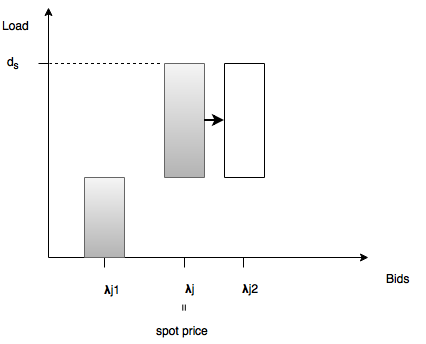
\includegraphics[scale=0.5]{../documentation/p1_c3.png}
\caption{Spot price equals to $\lambda_j$ bid. In this case, the production of $\lambda_j$ is needed to fulfil the demand so if we increase it to $\lambda_{s,j2}$ the spot price will follow. Since the spot price follows our bid $\lambda_{s,j2}$ at least, that means that the profit $R_s$ increases.}
\end{figure}
\end{itemize}
This proves that increasing the bid $\lambda_j$ to $\lambda_{s,j2}^c$ results in a constant profit or an increasing one. Therefore it is always better to select bid prices amongst all possible competitors bid prices.
Let us rewrite our problem with this new thought in mind. We introduce a competitor bid price $\lambda_i^c$ from any scenario replacing s,j with i for an arbitrary scenario and generator. It is important to remember that those prices are sorted in ascending order:\\
$\lambda_1^c < \lambda_2^c < ...< \lambda_n^c$\\ \\
This adds two new binary variables to the model: \\\\
$y_{s,i} = 1$ if the spot price in scenario $s$ is set to $\lambda_i^c$\\
$x_{ij} = 1$ if our bid $\lambda_j$ is equal to $\lambda_i^c$\\ \\
This allows us to rewrite the model as follows:\\
\begin{equation}
\max R, \\
\end{equation}
s.t.\\
\begin{equation}
R = \sum_{s \in S} p_s R_s
\end{equation}
\begin{equation}
 R_s = \sum_{j \in J} \left(\sum_{i \in I} y_{s,i} \lambda^c_i - c_j\right) g_{s,j} \ \ \  \forall s \in S
\end{equation}
The profit associated to a scenario equals the sum of the quantity bids multiplied by the difference of the bid prices chosen by the system operator and the production cost.
\begin{equation}
\bar{g}_j \ge 0 \ \ \ \forall s \in S, j \in J
\end{equation}
\begin{equation}
\bar{g}_j \le g^*_j \ \ \ \forall s \in S, j \in J
\end{equation}
The bids must be positive and inferior to the capacity of the generator.\\
\begin{equation}
x_{ij} \in \{0,1\} \ \ \  \forall i \in I, j \in J
\end{equation}
\begin{equation}
\sum_{i \in I} x_{ij} = 1 \ \ \  \forall j \in J
\end{equation}
\begin{equation}
y_{s,i} \in \{0,1\} \ \ \  \forall s \in S, i \in I
\end{equation}
\begin{equation}
\sum_{i \in I} y_{s,i} = 1 \ \ \ \forall s \in S
\end{equation}
By definition those 2 variables are boolean. The sum for $y_{s,i}$ means that there can only be one spot price per scenario and it is set at a competitor's bid price. The sum for $x_{ij}$ means that every bid $\lambda_j$ that we do must be equal to one of the competitors bid prices.\\
\begin{equation}
g_{s,j} \ge 0 \ \ \ \forall s \in S, j \in J
\end{equation}
\begin{equation}
g_{s,j} \ge \bar{g}_j x_{ij} y_{s,i'} \ \ \ \forall s \in S, j \in J \ \ i, i' \in I, i < i' \label{cons:notlin1}
\end{equation}
The quantity produced by a generator cannot be negative. If our bid price $\lambda_j$ is equal to the bid price of a competitor's bid price which is inferior to the spot price then the actual production for our generator j for the scenario s is superior or equal to our quantity bid made for it.\\
\begin{equation}
g_{s,j} \le \bar{g}_j \ \ \  \forall s \in S, j \in J
\end{equation}
\begin{equation}
g_{s,j} \le \bar{g}_j \left( 1 - x_{ij} y_{s,i'} \right) \ \ \  \forall s \in S, j \in J \ \ \  i, i' \in I, i > i' \label{cons:notlin2}
\end{equation}
The quantity produced by our generator is inferior or equal to our quantity bid for that generator. If our bid price $\lambda_j$ is equal to the bid price of a competitor's bid price which is superior to the spot price then the actual production for our generator j for the scenario s is zero.\\
\begin{equation}
\sum_{j \in J} g_{s,j} + \sum_{\substack{j \in J^c \\ \lambda^c_{s,j} < \lambda_i}} \bar{g}^c_{s,j} \le d^s y_{s,i} + \left(\max_{s' \in S} d^{s'} \right) (1 - y_{s,i})
\end{equation}
$\forall s \in S, i \in I$\\ \\
The sum of our quantities produced plus the sum of those from our competitors so that their price is inferior of this of $\lambda_i$ is inferior or equal to the demand for the specific scenario if our price bid is equal to this of our competitor or to the maximum demand of another scenario.
\begin{equation}
\sum_{j \in J} g_{s,j} + \sum_{\substack{j \in J^c \\ \lambda^c_{s,j} \le \lambda_i}} \bar{g}^c_{s,j} \ge d^s y_{s,i}\ \ \  \forall s \in S, i \in I
\end{equation}
The sum of our production plus the sum of quantities offered by the competitors so that their price is inferior or equal to $\lambda_i$ is either greater then the demand for the scenario s if our bid price is equal to this of the competitor or is otherwise simply positive.
We mentioned in our descriptions above that two of the constraints are not linear (\ref{cons:notlin1}) and (\ref{cons:notlin2}), luckily they involve binary variables and can be linearised:\\ \\
\begin{equation}
g_{s,j} \ge \bar{g}_j - g^*_j (2 - x_{ij} - y_{s,i'}) \ \  \forall s \in S, j \in J, i, i' \in I, i < i'\label{cons:lin1}
\end{equation}
\begin{equation}
g_{s,j} \le g^*_j (2 - x_{ij} - y_{s,i'}) \ \  \forall s \in S, j \in J, i, i' \in I, i > i'\label{cons:lin2}
\end{equation}\\\\
Since $x_{ij}$ and $y_{s,i}$ are boolean variables we can verify their validity with the following tables. We compare the constraint (1)and its linearisation(2)\\
For the first linearisation:\\ \\
(1) $g_{s,j} \geq \bar{g}_j \ x_{ij} \ y_{s,i'}$ (\ref{cons:notlin1})\\
(2) $g_{s,j} \ge \bar{g}_j - g^*_j (2 - x_{ij} - y_{s,i'})$ (\ref{cons:lin1})\\\\
\begin{tabular}{|c|c|c|}
  \hline
  \(\displaystyle y_{s,i'}|x_{ij} \) & 0 & 1 \\
  \hline
  0 & (1) \(\displaystyle g_{s,j} \geq \bar{g}_j - 2g^*_j \) & (1) \(\displaystyle g_{s,j} \geq 0 \) \\
   & (2) \(\displaystyle g_{s,j} \geq g_j - 2g^*_j \) & (2) \(\displaystyle g_{s,j} \geq \bar{g}_j - g^*_j \)\\
  \hline 
  1 & (1) \(\displaystyle g_{s,j} \geq 0 \) & (1)\(\displaystyle g_{s,j} \geq \bar{g}_j \) \\
   & (2)\(\displaystyle g_{s,j} \geq \bar{g}_j - g^*_j \) & (2)\(\displaystyle g_{s,j} \geq  \bar{g}_j\)\\
  \hline
\end{tabular}\\\\
For the second one:\\\\
(1) $g_{s,j} \le \bar{g}_j \left( 1 - x_{ij} y_{s,i'} \right)$ (\ref{cons:notlin2})\\
(2) $g_{s,j} \le g^*_j (2 - x_{ij} - y_{s,i'})$ (\ref{cons:lin2})\\\\
\begin{tabular}{|c|c|c|}
  \hline
  \(\displaystyle y_{s,i'}|x_{ij} \) & 0 & 1 \\
  \hline
  0 & (1) \(\displaystyle g_{s,j} \leq \bar{g}_j\) & (1) \(\displaystyle g_{s,j} \leq \bar{g}_j \) \\
   & (2) \(\displaystyle g_{s,j} \leq 2g^*_j \) & (2)\(\displaystyle g_{s,j} \leq g^*_j \)\\
  \hline
  1 & (1) \(\displaystyle g_{s,j} \leq \bar{g}_j \)  & (1)\(\displaystyle g_{s,j} \leq 0 \) \\
   & (2)\(\displaystyle g_{s,j} \leq g^*_j \) & (2)\(\displaystyle g_{s,j} \leq 0 \)\\
  \hline
\end{tabular}\\\\
We notice that for each case in the table we have valid and similar inequalities.\\\\
We also have to replace another term in one of the constraints in the definition of $R_s$, $\ $ $y_{s,i}g_{s,j}$ by $ \ yg_{s,ij}$ which follows the following constraints:\\
\begin{equation}
yg_{s,ij} \ge 0
\end{equation}
The production must always be positive.
\begin{equation}
yg_{s,ij} \le g_{s,j}
\end{equation}
Since $y_{s,i}$ is boolean, after setting its minimum to 0 with the precedent constraint, its maximum is when $y_{s,i}$ is equal to 1, which is equal to the production of the generator.\\
QUESTION pourquoi ne pas \'ecrire $0 < yg_{s,ij} \le g_{s,j}$ au lieu d'\'ecrire 2 contraintes ?
\begin{equation}
yg_{s,ij} \le g^*_j y_{s,i}
\end{equation}
The production  of a generator must always be capped by its capacity.
\begin{equation}
yg_{s,ij} \ge g_{s,j} - g^*_j (1 - y_{s,i})
\end{equation}
If the spot price is set to $\lambda_i^c$ then the production is equal to the quantity production decided. Otherwise our production must be inferior ro equal to the maximum capacity of the generator.\\
Je ne comprends pas tres bien l'interet de cette derniere contrainte vu qu'on dirait une combinaison des 3 autres.

\section{A relaxation of the problem}
Labb\'e etal[Mixed-Integer Programming Formulation] studied a new approach to the problem. Instead of considering that the generators can offer at most one amount at one price per generator, now the companies can offer bids with the capacities of all their generators combined.\\
Imagine 2 generators with the previous approach we could only do 2 bids, one per generator. With this approach we could do as many bids we wish without exceeding their capacity.\\
This already allows for improvement since we avoid the waste of generators not using their whole capacity.\\ Most importantly, they add another feature which is the stingy dispatching.\\
Generous dispatching used before meant that we would choose as spot price the first price corresponding to the quantity that would surpass the load needed. Now with this stingy dispatching we stop at the first price reaching the load needed. \\
This might not seem like a drastic change but this allows us to completely rewrite the problem. The new idea is that we can construct a solution satisfying M. Fampa's generous dispatching assumption by reducing infinitesimally our quantity corresponding to the spot prices: \\\\
\textbf{The load dispatching}
\begin{figure}[!ht]
\centering
\textbf{Generous solution}\par\medskip
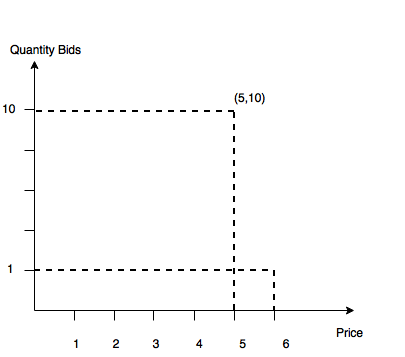
\includegraphics[scale=0.45]{../documentation/Generous.png}
\caption{Load = 10, so the system controller will stop at the first price where the load is met. Here, one of the companies offers 10 quantities at the lowest price 5 and the other 1 quantity at 6. The first one has the lowest price and fulfils the needs of the operator therefore they sell their 10 quantities of energy at 5.}
\end{figure}
\begin{figure}[!ht]
\centering
\textbf{Stingy solution}\par\medskip
\includegraphics[scale=0.45]{../documentation/Stingy.png}
\caption{Same problem, but the company offers 9,99 instead of 10 therefore the spot price is fixed at the next price reaching the load which is 6, this way the company can sell the same amount of energy at a higher price.}
\end{figure}

The relaxation of the problem we consider assumes that for each generator can be any arbitrary number of bids. Bids are not related to specific generators any more. Each bid is now associated to a price $\lambda_i$.
Therefore we need a new notations and variables:\\
\begin{tabular}{ll}
$g_i$ & The quantity bid on price $\lambda_i$\\
\(\displaystyle G_i = \sum_{\substack{i' \in I\\i'\le i}} g_{i'}\) & Cumulative bid quantities\\
\(\displaystyle r_{s,i} = d_s - \sum_{\substack{j \in J^c\\ \lambda^c_{s,j} < \lambda_i}} \bar{g}^c_{s,j} \) & The residual demands \\
\(\displaystyle c^e_i = \sum_{\substack{j \in J\\c_j < \lambda_i}} g^*_j \) & The effective capacities\\
\end{tabular}\\ \\
From now on, the $G_i$ will be used instead of the $g_i$, with the following restrictions:\\
\begin{tabular}{ll}
$G_{i'} \ge G_i$ if $i'>i$ & Negative bid quantities are not allowed\\
$G_i \le c^e_i$ & Production at loss is not allowed \\
\end{tabular}
\subsection{Proposition 2 - impact on profit}
The impact on profit by modifying a consecutive list of cumulative bid quantities $\{G_i, ...., G_{i'} \}$ only depends on the modified quantities and their neighbouring quantities $G_{i-1}$ and $G_{i'+1}$.
\subsection{Proof}
We are going to evaluate the effect on an arbitrary scenario of the modifications of those cumulative bid quantities. Let us see how the profit $R_s$ reacts to those modifications. There are three possible cases:\\
\begin{itemize}
\item $G_{i-1} > r_{s,i}$: \\
The demand is provided by the lower generators therefore the spot price $\pi_d^s$ is lower than $\lambda_i \ \rightarrow \ R_s$ is constant.
\item $G_{i'+1} \le r_{s,i'+1}$: \\
The last value of the packet of quantity bids is lower than the spot price $\pi_d^s \ \rightarrow \ \pi_d^s$ does not depend on them and the production neither because they are already all sold. $R_s$ stays constant.
\item $G_{i-1} \le r_{s,i} \wedge G_{i'+1} > r_{s,i'+1}$: \\
Since the demand is not satisfied under $\lambda_i$ but is for $\lambda_i'$, the spot price is between those 2 values therefore a modification of those values does influence the profit.
\end{itemize}
We realize that the profit is a function of the modified cumulative bid quantities and their two neighbouring values. The function is the following: \\
\(\displaystyle R\left( (\lambda_1, g_1), \ldots, (\lambda_n, g_n) \right) =
R\left( (\lambda_1, g_1) \right) +
\sum_{k=2}^n \left[ R\left( (\lambda_{k-1}, G_{k-1}), (\lambda_k, g_k) \right) -
R\left( (\lambda_{k-1}, G_{k-1}) \right) \right].\) 
\subsection{Proposition 3 - Thresholds}
At least one of the set of optimal bids has all the $G_i$ equal to one of the possible thresholds.
The possible thresholds : \\
\begin{itemize}
\item The effective capacity $c_i^e \ \rightarrow \ $ we do not want to either be above or under it.
\item The residual demand for the next higher bid price if lower than $c_i^e$.
\item The bid quantity equal to following one is at threshold. $G_i = G_{i+1}$.
\end{itemize}
\subsection{Proof}
We can show that if we have a solution we can always improve it by moving one of the $G_i$  as long as all the $G_i$ are not at thresholds.\\
There are 2 cases to consider:\\
\begin{itemize}
\item $G_i > c^e_i$\\
In this case we produce more than what effective, this means we can reduce $G_i$ to $c^e_i$ and increase our profit or leave it unchanged.
\item $G_i < c^e_i$\\
If $G_i$ is not at any precedent threshold and $G_i < G_{i+1}$. we can always find $i$ so that $i'$ is not at threshold. In that case, the profit value obtained by increasing $G_i$ to its next thresholds will depend on the spot price:\\
\begin{itemize}
\item $\pi_s < \lambda_i$: All the demand is already covered, $R_s$ stay unchanged after increasing $G_i$.
\item $\pi_s > \lambda_{i+1}$: We need at least to reach $\lambda_{i+2}$ to reach the spot price. Since we cannot bid higher than $G_{i+1}$ this means that increasing $G_i$ will not change the value of the spot price. As a consequence $R_s$ stays unchanged.
\item $\pi_s = \lambda_i$: The demand needs the production at $\lambda_i$. We face 2 cases:\\
\begin{itemize}
\item $G_i < r_{s,i} \ \rightarrow \ $ Increasing $G_i$ increases our selling therefore increasing our profit.
\item $G_i \geq r_{s,i}\ \rightarrow \ $ This means that we reached the maxima, implying that increasing will not increase our selling and our profit.\\
\end{itemize}
In both cases the spot prices stays at $\lambda_i$.
\item $\pi_s = \lambda_{i+1}$: We visualize here a possible loss in profit. The spot price could decrease if the following happens, $G_i > r_{s,i}$. But $r_{s,i}$ is a threshold, and as a result $G_i$ cannot be increased passed it. This means that the spot price remains constant and so increasing $G_i$ does not impact the profit.
\end{itemize}
\end{itemize}
This proves that an optimal set of bids can be found where the $G_i$ take specific values(thresholds). There are a finite number of thresholds and we can find the optimal solution in finite time. 
\subsection{Implementation of the shortest path}
After what we learned from the third proposition, we are now looking to create the algorithm to solve the problem. The issue is that such algorithm takes an exponential time. Here is where the second proposition comes to play, "since the profit function $R$ can be written as an incremental sum over individual bids, we can optimise each bid iteratively".\\
We define $R_i^{max}(G_i) \ \rightarrow \ $ The maximum profit when bidding for a total quantity $G_i$ at price up to $\lambda_i$.\\ \\
\(\displaystyle R^{max}_i(G_i) = \max_{\substack{G_{i-1} \in \left\{ c^e_{i-1}, G_i \right\}
\cup \left\{ r_{s,i} \forall s \in S \right\}\\ 0 \le G_{i-1} \le G_i}}
R^{max}_{i-1}(G_{i-1}) +
\left[  R\left( (\lambda_{i-1}, G_{i-1}), (\lambda_i, G_i - G_{i-1}) \right) -
R\left( (\lambda_{i-1}, G_{i-1}) \right) \right]. \) \\ \\
The optimal profit is obtained with $R_i^{max}(c_i^e)$ associated with the highest bid value of the problem.\\ \\
"The single-scenario single-bid profit function $R_s((\lambda_i, G_i))$
has three regimes: none of the bid is sold, a partial amount of is sold
at the value given, or all of it is sold at a potentially higher spot price."\\
\(\displaystyle R_s((\lambda_i, G_i)) = \left\{
	\begin{array}{cl}
	0 & \mbox{if } r_{s,i} < 0, \\
	\lambda_i r_{s,i} - c(r_{s,i}) & \mbox{if } 0 \le r_{s,i} < G_i, \\
	G_i \left( \min_{i' \ge i} \left\{ \lambda_{i'} : r_{s,i'+1} < G_i \right\} \right)\\ - c(G_i) & \mbox{if } G_i \le r_{s,i}.
	\end{array}
\right.\)
\\ \\ 
Definition of the new variable and functions:\\
\begin{tabular}{ll}
$c(G)$ & The total of production for G  units of energy. \\
$c(r_{s,i})$ & The total cost of the residual demands.\\
\end{tabular}\\ \\
The tactic used to speed up the calculation of our optimal profit is by pre-calculating these profit function($R_s((\lambda_i, G_i))$), afterwards we use those pre-calculations to calculate the profit increments.\\ \\
\(\displaystyle R_s\left( (\lambda_{i-1}, G_{i-1}), (\lambda_i, G_i - G_{i-1}) \right) -
R_s((\lambda_i, G_i)) = \left\{
	\begin{array}{cl}
	0 & \mbox{if } r_{s,i} < G_{i-1}, \\
	R_s((\lambda_i, G_i)) - R_s((\lambda_{i-1}, G_{i-1})) & \mbox{if } G_{i-1} \le r_{s,i}.
	\end{array}
\right. \)\\ \\
This is where we finally visualize the shortest path part of the algorithm. This last formula can be understood easily, there are two choices when adding an additional bid to a previous bid:\\
\begin{itemize}
\item Either there is no demand at the new bid price and the additional bid does not change the system ($r_{s,i} < G_{i-1}$).
\item Or there is some demand to be fulfilled at the new bid price and the spot price will at least be at that value ($G_{i-1} \le r_{s,i}$).
\end{itemize}
\section{The algorithm}
\end{document}
